\documentclass[11pt]{article}
\usepackage{fullpage}
\usepackage{graphics,epsfig,color}
\usepackage{wrapfig}
\usepackage{times}
\usepackage{setspace}
\usepackage{amsmath,amsthm,amssymb}
\usepackage{url}
\usepackage{fancyhdr}
\usepackage{enumitem}
\pagestyle{fancy}


\newtheorem{theorem}{Theorem}[section]
\newtheorem{corollary}{Corollary}[section]
\newtheorem{lemma}{Lemma}[section]
\newtheorem{problem}{Problem}
\newtheorem{definition}{Definition}[section]
\newtheorem{observation}{Observation}[section]
\newtheorem{example}{Example}[section]
\newtheorem{openproblem}{Open Problem}[section]
\newtheorem{fact}{Fact}[section]

\newcommand{\qedsymb}{\hfill{\rule{2mm}{2mm}}}
\newenvironment{proofsketch}
{
	\begin{trivlist}
	\item[\hspace{\labelsep}{\noindent Proof Sketch: }]
}{\qedsymb\end{trivlist}}



%the following few lines until usepackage{algorithm2e} is to avoid the
%conflicts of algorithm2e with other packages.
\makeatletter
\newif\if@restonecol
\makeatother
\let\algorithm\relax
\let\endalgorithm\relax
\usepackage[ruled,vlined,linesnumbered]{algorithm2e}

\newcommand{\remove}[1]{}



%--------------------------------


\begin{document}

	\renewcommand{\headrulewidth}{0.4pt}
	\setlength{\headheight}{38.0pt}
	\fancyhead[L]{\bf CSCD300 Homework 6, Winter 2012, 
	Eastern Washington University. Cheney, Washington. \\
	\bigskip Name: Eric Fode\hspace{40mm}EWU ID:00530214}


	\noindent{\bf Solution for Problem 1}\\
	The lower bound of the number of leaf nodes occur when all the nodes in the tree
	have exactly one child. In this case there will be only 1 leaf node. \\
	The upper bound of the number of leaf nodes occurs when the tree is full in which 
	case the tree will have $n/2$ leaf nodes. 

	
	\noindent{\bf Solution for Problem 2}\\
	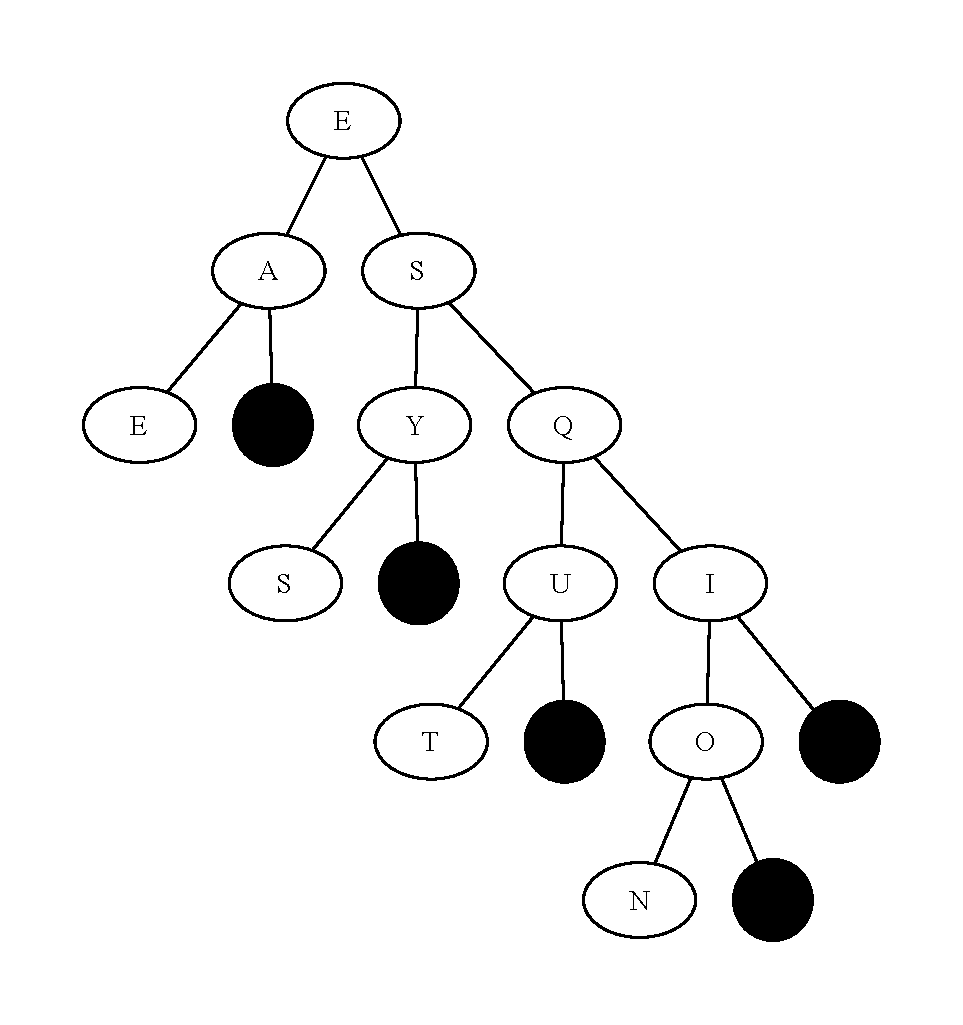
\includegraphics[scale=1]{bst.pdf}\\
		
	\newpage
	\noindent{\bf Solution for Problem 3}\\
	meet me later\\
	
	\bigskip
	\noindent{\bf Solution for Problem 4}\\
	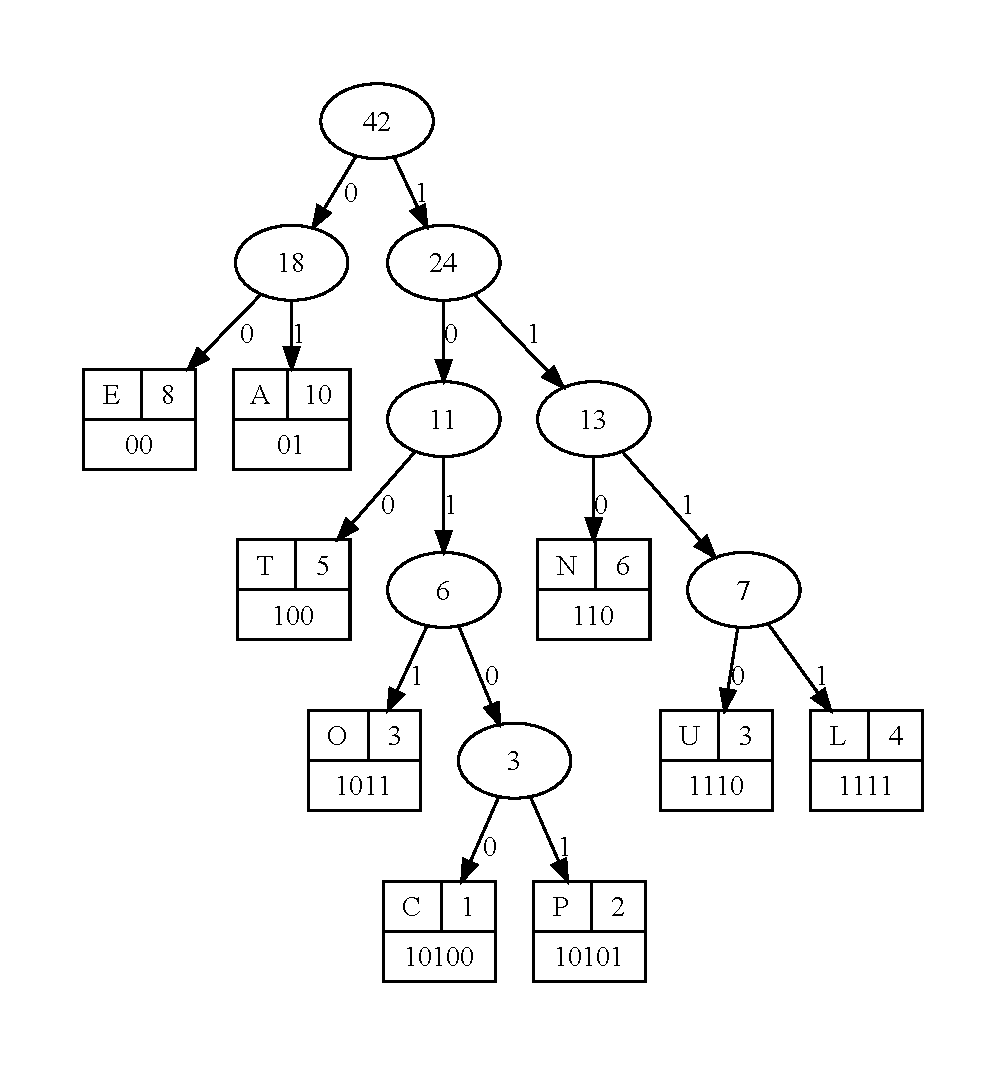
\includegraphics[scale=1]{huffman.pdf}\\
	
	\newpage
	\noindent{\bf Solution for Problem 5}\\
	1010001110100011111101111101010100\\
	
\end{document}